\subsection{Usar el complemento GPS}\label{label_plugingps}

\subsubsection{¿Qué es GPS?}\label{whatsgps}

GPS, el Sistema de Posicionamiento Global, es un sistema basado en satélites que permite a cualquiera con un receptor GPS conocer su posición exacta en cualquier parte del mundo. Se usa como ayuda en navegación, por ejemplo para aviones, en barcos y por excursionistas. El receptor GPS utiliza la señal de los satélites para calcular su latitud, longitud y (en ocasiones) altura. La mayoría de los receptores tiene también la capacidad de guardar localizaciones (conocidas como \emph{waypoints}), secuencias de localizaciones que forman una \emph{ruta} planeada y un registro de recorridos o \emph{track} de los movimientos del receptor a lo largo del tiempo. Waypoints, rutas y tracks son los tres tipos de elementos básicos en los datos de GPS. QGIS muestra los waypoints en capas de puntos, mientras que las rutas y tracks se muestran en capas de líneas.

\subsubsection{Cargar datos GPS de un archivo}\label{label_loadgps}

Existen docenas de formatos de archivo diferentes para guardar datos de GPS. El formato utilizado por QGIS se llama GPX (GPS eXchange format-Formato de intercambio GPS), que es un formato estándar de intercambio que puede almacenar cualquier número de waypoints, rutas y tracks en el mismo archivo.

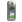
\includegraphics[width=0.7cm]{icon} Para cargar un archivo GPX necesita usar el complemento \emph{Herramientas GPS}. Cuando se carga este complemento aparece un botón con un pequeño dispositivo GPS de mano en la barra de herramientas (el dispositivo se parece un poco a un teléfono móvil). Pulsando en este botón se abrirá el diálogo \emph{Herramientas GPS} (vea la Figura \ref{figure GPX loader}).

\begin{figure}[ht]
   \begin{center}
\caption{\label{figure GPX loader}La ventana del diálogo \emph{Herramientas GPS}}
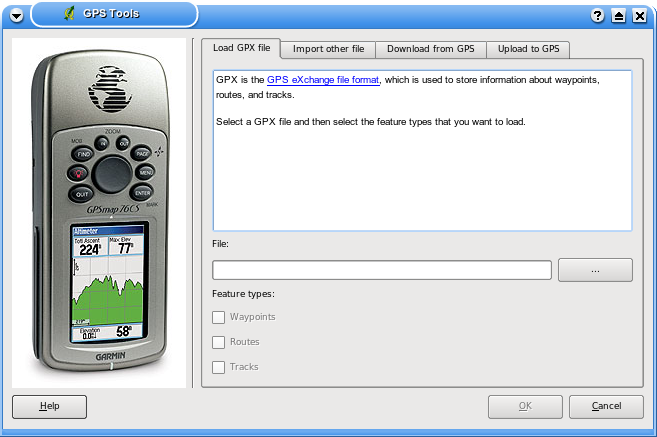
\includegraphics[clip=true, width=16cm]{loadgpx}
\end{center}
\end{figure}

Utilice el botón {[}Explorar...{]} para seleccionar el archivo GPX y luego use las casillas de verificación para seleccionar el tipo de objeto espacial que quiere cargar de ese archivo GPX. Cada tipo de objeto espacial se cargará en una capa diferente cuando pulse Aceptar.

\subsubsection{GPSBabel}

Puesto que QGIS utiliza archivos GPX, necesita una forma de convertir otros formatos de archivo de GPS a GPX. Esto lo puede hacer para muchos formatos usando el programa libre GPSBabel, que está disponible en \url{http://www.gpsbabel.org}. Este programa también puede transferir datos de GPS entre su equipo y un dispositivo GPS. QGIS utiliza GPSBabel para hacer estas cosas, por lo que se recomienda que lo instale. Sin embargo, si solamente quiere cargar datos de GPS desde archivos GPX no lo necesitará. La versión 1.2.3 de GPSBabel se sabe que funciona con QGIS, pero debería poder usar versiones posteriores sin problemas.


\subsubsection{Importar datos de GPS}

Para importar datos de GPS de un archivo que no sea GPX se usa la herramienta  \emph{Importar otro archivo} del diálogo \emph{Herramientas GPS}. Aquí seleccione el archivo que quiera importar, el tipo de objeto espacial que quiera importar de él, dónde quiere guardar el archivo convertido a GPX y cuál debe ser el nombre de la nueva capa.

Cuando seleccione el archivo a importar también debe seleccionar el formato
del archivo usando el menú del diálogo de selección de archivo (vea la figura
\ref{figure importdialog}). No todos los formatos soportan los tres tipos de
objetos espaciales, por lo que para muchos formatos sólo podrá seleccionar uno o 
dos tipos.

\begin{figure}[ht]
   \begin{center}
\caption{\label{figure importdialog}Diálogo de selección de archivo de la herramienta de importación}
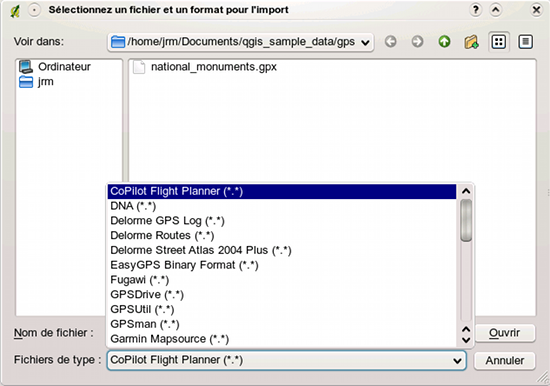
\includegraphics[clip=true, width=12cm]{importdialog}
   \end{center}
\end{figure}

\subsubsection{Descargar datos de GPS desde un dispositivo}

QGIS puede usar GPSBabel para descargar datos desde un receptor GPS
directamente a capas vectoriales. Para ello utilice la herramienta \emph{Descargar desde GPS} (vea la Figura \ref{figure_download}), donde se selecciona el tipo de dispositivo GPS, el puerto al que está conectado, 
el tipo de objeto espacial que quiere descargar, el archivo GPX donde se deben
guardar los datos y el nombre de la nueva capa.

\begin{figure}[ht]
   \begin{center}
\caption{\label{figure_download}La herramienta descargar}
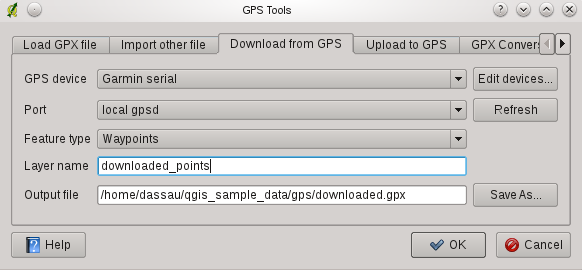
\includegraphics[clip=true, width=16cm]{download}
   \end{center}
\end{figure}


El tipo de dispositivo que seleccione en el menú de receptores GPS determina la forma en la que GPSBabel
intenta comunicarse con él. Si no funciona ninguno de los tipos de dispositivo con su receptor GPS puede crear un nuevo tipo (vea la sección
\ref{sec:Defining-new-device}).

El puerto es un nombre de archivo u otro nombre que utilice su sistema operativo
como referencia del puerto físico de su ordenador al que
está conectado el dispositivo GPS. En Linux esto es algo como /dev/ttyS0
o /dev/ttyS1 y en Windows es COM1 o COM2.

Cuando pulse Aceptar los datos se descargarán desde el receptor y aparecerán como una capa en QGIS.

\subsubsection{Cargar datos de GPS a un dispositivo}

También puede cargar datos directamente desde una capa vectorial de QGIS a
un dispositivo GPS, usando la herramienta \emph{Cargar a GPS}. La capa debe ser una capa GPX.
Para hacer esto simplemente seleccione la capa que quiera cargar, el tipo de su
dispositivo GPS y el puerto al que esté conectado. Igual que con la herramienta descargar, 
puede especificar nuevos tipos de dispositivo si el suyo no está en la lista.

Esta herramienta es muy útil junto con las capacidades de edición de capas 
vectoriales de QGIS. Puede cargar una mapa, crear algunos waypoints y rutas y
luego cargarlos y usarlos en su dispositivo GPS.

\subsubsection{\label{sec:Defining-new-device}Definir nuevos tipos de dispositivo}

Existen numerosos tipos distintos de receptores GPS. Los desarrolladores de
QGIS no puede probarlos todos, por lo que si tiene uno que no funciona con 
ninguno de los tipos listados en las herramientas de descarga y carga puede 
definir su propio tipo. Esto se hace usando el \emph{editor de receptores GPS}, 
que puede iniciar pulsando el botón \emph{Editar receptores} en las
ventanas de descarga o carga.

Para definir un receptor nuevo simplemente pulse el botón \emph{Nuevo receptor},
introduzca un nombre, una orden de descarga y una orden de carga para su dispositivo 
y pulse el botón \emph{Actualizar receptor}. El nombre, que puede ser cualquier cadena, aparecerá en la lista
de receptores en las ventanas de carga y descarga.

La orden de descarga es la que se usa para descargar datos desde un 
receptor a un archivo GPX. Probablemente será una orden de GPSBabel, pero
puede usar cualquier otro programa de línea de órdenes que pueda crear un 
archivo GPX. QGIS sustituirá las palabras clave \emph{\%type}, \emph{\%in} y
\emph{\%out} cuando ejecute la orden.

\emph{\%type} se sustituirá por {}``-w'' si está descargando waypoints, por {}``-r''
 si está descargando rutas y por {}``-t'' si está descargando tracks. Estas son opciones
 de línea de órdenes que le dicen a GPSBabel qué tipos de objetos espaciales descargar.

\emph{\%in} se sustituirá por el nombre del puerto que elija en la ventana de
descarga y \emph{\%out} se sustituirá por el nombre que elija para el archivo
GPX en el que se guardarán los datos descargados. Así, si crea un tipo de 
dispositivo con la orden de descarga {}``gpsbabel
\%type -i garmin -o gpx \%in \%out'' (esta es en realidad la orden de descarga 
para el tipo de receptor predefinido {}``Garmin serie'') y lo usa para descargar 
waypoints del puerto {}``/dev/ttyS0'' al archivo {}``output.gpx'', QGIS sustituirá 
las palabras clave y ejecutará la orden {}``gpsbabel -w -i garmin -o gpx /dev/ttyS0 output.gpx''.

La orden de carga es la que se usa para cargar datos al receptor. Se utilizan 
las mismas palabras clave, pero \emph{\%in} ahora se sustituye por el nombre del 
archivo GPX de la capa que se está cargando y \emph{\%out} se sustituye por el nombre 
del puerto. Puede aprender más sobre GPSBabel y sus opciones de línea de órdenes en 
\url{http://www.gpsbabel.org}

Una vez que haya creado un tipo de receptor nuevo, aparacerá en la lista de dispositivos de las herramientas de descarga y carga.